% Revisão OK 12/10
\chapter{Modelo de Dados}

Nesta seção, explica-se o modelo de dados desenvolvido para o projeto, abordando 
sua estrutura lógica e os componentes principais. O objetivo deste modelo é garantir 
flexibilidade para futuras alterações e manutenções, proporcionando uma base sólida 
e expansível para o projeto.

\section{Modelo Lógico}

O modelo de dados foi feito de forma que futuras alterações possam ser absorvidas 
facilmente. Abaixo está o diagrama entidade-relacionamento, no qual o nome no topo 
do retângulo identifica o nome da tabela. A lista abaixo do nome mostra as colunas 
dessas tabelas, a sigla PK denota \textit{chave primária} e FK \textit{chave estrangeira}.

Uma relação é denotada pelas setas ligando duas tabelas. A cardinalidade da relação é indicada
pelos números entre parênteses. 

Para a relação \texttt{Aerodrome-ILS}, temos (1, 1) para (0, n), significando que 
um aeródromo pode ter zero ou mais frequências de ILS e esta só pode ser de um único 
aeródromo.

Já na relação \texttt{Aerodrome} com \texttt{Runway}, um aeródromo deve ter \texttt{uma ou mais} pistas
e uma pista pertence a um único aeródromo.

\pagebreak

\begin{figure}[ht]
    \begin{center}
    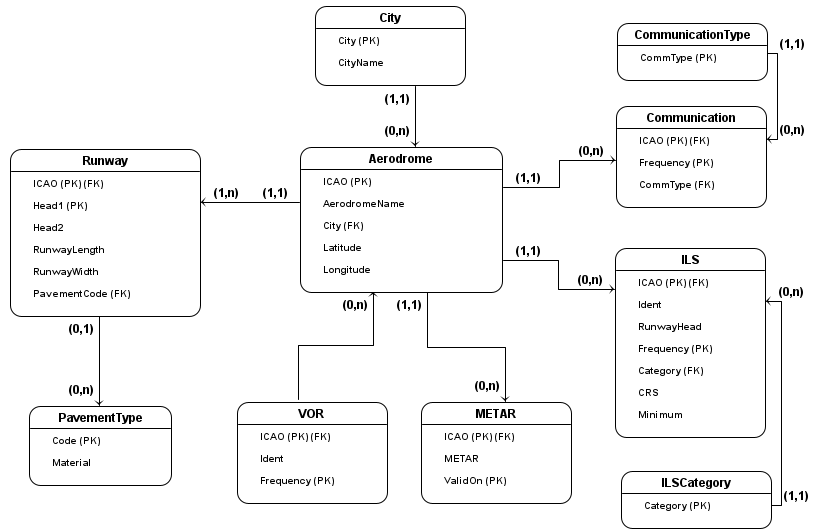
\includegraphics[width=400pt]{img/ERAero.png}
    \caption{Diagrama lógico}
    \label{fig:diagrama-er}
    \end{center}
\end{figure}

Note-se que as tabelas "CommunicationType", "ILSCategory" e "PavementType" poderiam 
ser substituídas por colunas enum nas tabelas "Communication", "ILS" e "Runway", 
porém a manutenção seria difícil \cite{table-enum}, pois teríamos que alterar a 
estrutura das tabelas (possivelmente tirando o Aero do ar) caso fosse necessário 
adicionar um tipo novo de comunicação, por exemplo. Fazendo com uma tabela externa 
é necessário apenas adicionar uma nova linha.

\section{Noções sobre o Funcionamento de um Aeródromo}

Antes de discutir as tabelas, é interessante compreender algumas regras e 
características básicas do funcionamento de um aeródromo. Isto certamente
facilitará o entendimento das colunas das tabelas.

Um aeródromo é a área destinada às operações de pouso, decolagem, e taxiamento 
de aeronaves, abrangendo pátio, taxiways (vias de taxi) e pistas. O terminal de 
passageiros, no entanto, não faz parte do aeródromo em si. Por isso, todos os 
aeroportos são aeródromos, mas nem todo aeródromo é um aeroporto, pois nem todos 
possuem infraestrutura para o atendimento de passageiros.

\subsection{Pistas}

Para o entendimento do funcionamento das pistas de pouso e decolagem, é importante 
conhecer algumas de suas características essenciais, como comprimento e largura, 
que impactam diretamente as operações das aeronaves.

O comprimento da pista, por exemplo, influencia a quantidade de frenagem necessária 
para uma aeronave parar com segurança após o pouso. Em pistas curtas, certos 
modelos de aeronaves não podem pousar com segurança. Já a largura da pista limita 
a envergadura máxima das aeronaves que podem operar nela. Em pistas muito estreitas, 
uma aeronave de grande porte, como o Boeing 747, pode ter dificuldades adicionais: 
os motores mais externos podem ultrapassar a área pavimentada, expondo-os a 
materiais no gramado, o que aumenta o risco de ingestão de objetos.

No caso de cabeceiras paralelas, ou seja, pistas que apontam para a mesma direção, 
temos as seguintes configurações:

\subsubsection{Pista Única}

A numeração da cabeceira da pista é determinada pela sua orientação magnética, 
dividida por 10 e arredondada. Por exemplo, em Fortaleza, a cabeceira com 
orientação de 126 graus é numerada como 13 (126 dividido por 10 é igual a 
12,6, que arredondamos para 13).

\subsubsection{Pista Dupla}

Para pistas paralelas duplas, são usadas as letras "L" (Left, esquerda) e "R" 
(Right, direita) para distinguir as cabeceiras. No aeroporto Santos Dumont, por 
exemplo, temos as cabeceiras 02L (esquerda) e 02R (direita), quando o observador 
está de costas para o Pão de Açúcar.

\subsubsection{Pista Tripla}

Embora no Brasil não haja aeroportos com três pistas paralelas, em outros países, 
onde existem pistas triplas, são utilizadas as letras "L" (left/esquerda), "C" 
(center/central) e "R" (right/direita) para identificação das cabeceiras.

\subsection{Comunicação}

As frequências de comunicação em aeródromos utilizam modulação de amplitude (AM), com banda 
de 118 MHz a 137 MHz. Cada aeródromo possui frequências específicas para cada fase 
do voo, como autorização, taxi, decolagem, aproximação e pouso.

Os tipos de frequência achadas em aeroportos do Brasil são:

\begin{enumerate}
\item Tráfego
\item Torre
\item Solo
\item Rampa
\item ATIS
\item Operações
\end{enumerate}

Nesta trabalho, para cada aeroporto, são mostradas as frequencias usadas com seus
tipos.

\subsection{Navegação}

As frequências de navegação são utilizadas pelos sistemas de localização do avião, 
não transmitindo áudio, mas sim dados, dentro da faixa de 108 a 117.95 MHz. Esses 
sistemas ajudam a determinar a posição e a trajetória da aeronave com precisão.

\begin{itemize} 
\item VOR (Very High Frequency Omnidirectional Range): Um sistema 
de navegação baseado em uma antena no solo, o VOR permite que a aeronave 
determine a direção que deve seguir para passar diretamente sobre a antena, 
indicando essa direção em um instrumento específico na cabine. Na aviação isto
é chamado de bloqueio de VOR. \cite{vor-block}

\item ILS (Instrument Landing System): Sistema de aterrissagem por instrumentos 
que transmite informações de orientação lateral (alinhamento com o eixo da pista) 
e orientação vertical (ângulo de descida) específicas para cada cabeceira da pista. 
Essas informações permitem uma aproximação precisa, mesmo em condições de baixa 
ou nenhuma
visibilidade. O ILS pode ser usado tanto para pouso manual, onde o piloto controla
a aeronave seguindo 
as indicações, quanto para pouso automático (auto land), caso a aeronave possua 
esta capacidade. \cite{ils-train}
\end{itemize}

Neste trabalho são mostradas as frequências de ILS e VOR para cada aeroporto.

\section{Dicionário de Dados}

\begin{longtable}{|p{3.2cm}|p{6.4cm}|p{3cm}|}
    \caption{State} \\
    \hline
    \textbf{Nome} & \textbf{Descrição} & \textbf{Tipo} \\ \hline
    \endfirsthead
    \multicolumn{3}{c}%
    {{\tablename\ \thetable{} -- Continuação da página anterior}} \\
    \hline
    \textbf{Nome} & \textbf{Descrição} & \textbf{Tipo} \\ \hline
    \endhead
    \hline \multicolumn{3}{|r|}{{Continua na próxima página}} \\ \hline
    \endfoot
    \hline
    \endlastfoot
        StateCode (PK)
        & Código do IBGE \cite{IBGE-cidade} do estado
        & INTEGER
        \\ \hline
        StateName
        & Nome do estado escrito em Português com a primeira letra maiúscula
        & VARCHAR (50)
        \\ \hline
        StateAbbreviation
        & Abreviatura de duas letras do estado. Ambas as letras maiúsculas.
        & VARCHAR(2)
        \\ \hline
\end{longtable}

\begin{longtable}{|p{3cm}|p{6.6cm}|p{3cm}|}
    \caption{City} \\
    \hline
    \textbf{Nome} & \textbf{Descrição} & \textbf{Tipo} \\ \hline
    \endfirsthead
    \multicolumn{3}{c}%
    {{\tablename\ \thetable{} -- Continuação da página anterior}} \\
    \hline
    \textbf{Nome} & \textbf{Descrição} & \textbf{Tipo} \\ \hline
    \endhead
    \hline \multicolumn{3}{|r|}{{Continua na próxima página}} \\ \hline
    \endfoot
    \hline
    \endlastfoot
        CityCode (PK)
        & Código do IBGE \cite{IBGE-cidade} da cidade
        & INTEGER
        \\ \hline
        CityName
        & Nome da cidade escrito em Português com a primeira letra maiúscula
        & VARCHAR (50)
        \\ \hline
        StateCode (FK)
        & Chave estrangeira para o estado
        & INTEGER
        \\ \hline
\end{longtable}


\begin{longtable}{|p{3cm}|p{6.6cm}|p{3cm}|}
    \caption{Aerodrome} \\
    \hline
    \textbf{Nome}       & \textbf{Descrição} & \textbf{Tipo}  \\ \hline
    \endfirsthead
    \multicolumn{3}{c}%
    {{\tablename\ \thetable{} -- Continuação da página anterior}} \\
    \hline
    \textbf{Nome}       & \textbf{Descrição} & \textbf{Tipo}  \\ \hline
    \endhead
    \hline \multicolumn{3}{|r|}{{Continua na próxima página}} \\ \hline
    \endfoot
    \hline
    \endlastfoot
        ICAO (PK)
        & O código ICAO do aeródromo emitido pela Organização Internacional de Aviação Civil (ICAO).
        & VARCHAR(4)
        \\ \hline

        AerodromeName
        & O nome do aeródromo conforme definido pelo AISWEB, sistema nacional de informações aeronáuticas.
        & VARCHAR(50) 
        \\ \hline

        City (FK)
        & Chave estrangeira para o código da cidade
        & INTEGER
        \\ \hline

        Latitude 
        & A latitude do aeroporto em graus no formato de graus decimais (DD, Decimal Degrees). Três dígitos para 
        representar a parte inteira e seis dígitos para a fracionária.
        & DECIMAL(9, 6)
        \\ \hline
        
        Longitude 
        & A longitude do aeroporto, seguindo o mesmo formato da latitude. 
        & DECIMAL(9, 6)
        \\ \hline

        IsPublished 
        & Se for falso o aeródromo não aparece no site. Serve para que os aeródromos
        recém-criados não apareçam enquanto outras informações ainda não foram cadastradas.
        & Boolean
        \\ \hline
\end{longtable}

\begin{longtable}{|p{3cm}|p{6.6cm}|p{3cm}|}
    \caption{METAR} \\
    \hline
    \textbf{Nome}       & \textbf{Descrição} & \textbf{Tipo}  \\ \hline
    \endfirsthead
    \multicolumn{3}{c}%
    {{\tablename\ \thetable{} -- Continuação da página anterior}} \\
    \hline
    \textbf{Nome}       & \textbf{Descrição} & \textbf{Tipo}  \\ \hline
    \endhead
    \hline \multicolumn{3}{|r|}{{Continua na próxima página}} \\ \hline
    \endfoot
    \hline
    \endlastfoot
        ICAO (PK) (FK)
        & Chave estrangeira para qual aeródromo este METAR se refere
        & VARCHAR(4)
        \\ \hline

        METAR
        & O METAR em si
        & VARCHAR(100)
        \\ \hline

        ValidOn (PK)
        & \textit{Timestamp} com o momento que este METAR é válido. É construído a
        partir do item do metar "ddhhmmZ" em que "dd" é o dia e "hhmm" é
        a hora zulu (UTC). O mês e ano são o mês e ano atuais do sistema.
        & DATETIME

        \\ \hline
\end{longtable}

\begin{longtable}{|p{3cm}|p{6.6cm}|p{3cm}|}
    \caption{TAF} \\
    \hline
    \textbf{Nome}       & \textbf{Descrição} & \textbf{Tipo}  \\ \hline
    \endfirsthead
    \multicolumn{3}{c}%
    {{\tablename\ \thetable{} -- Continuação da página anterior}} \\
    \hline
    \textbf{Nome}       & \textbf{Descrição} & \textbf{Tipo}  \\ \hline
    \endhead
    \hline \multicolumn{3}{|r|}{{Continua na próxima página}} \\ \hline
    \endfoot
    \hline
    \endlastfoot
        ICAO (PK) (FK)
        & Chave estrangeira para qual aeródromo este TAF se refere
        & VARCHAR(4)
        \\ \hline

        TAF
        & O TAF em si
        & VARCHAR(100)
        \\ \hline

        ValidOn (PK)
        & \textit{Timestamp} com o momento que este TAF é válido. É construído a
        partir do item do TAF "ddhhmmZ" em que "dd" é o dia e "hhmm" é
        a hora zulu (UTC). O mês e ano são o mês e ano atuais do sistema.
        & DATETIME

        \\ \hline
\end{longtable}


\begin{longtable}{|p{3cm}|p{6.6cm}|p{3cm}|}
    \caption{PavementType} \\
    \hline
    \textbf{Nome}       & \textbf{Descrição}                                                                                          & \textbf{Tipo} \\ \hline
    \endfirsthead
    \multicolumn{3}{c}%
    {{\tablename\ \thetable{} -- Continuação da página anterior}} \\
    \hline
    \textbf{Nome}       & \textbf{Descrição}                                                                                          & \textbf{Tipo} \\ \hline
    \endhead
    \hline \multicolumn{3}{|r|}{{Continua na próxima página}} \\ \hline
    \endfoot
    \hline
    \endlastfoot

        Code (PK)
        & O código (em Inglês) do tipo de pavimento usado. É formado por três letras maiúsculas.
        & VARCHAR(3)
        \\ \hline

        Material 
        & O nome do pavimento em Português, com a primeira letra maiúscula.
        & VARCHAR(20)
        \\ \hline


\end{longtable}

\begin{verbatim}
Exemplo de siglas:

Code    Material
ASP     Asfalto
CON     Concreto
GVL     Brita
\end{verbatim}


\begin{longtable}{|p{3cm}|p{6.6cm}|p{3cm}|}
    \caption{Runway} \\
    \hline
    \textbf{Nome}       & \textbf{Descrição}                                                                                          & \textbf{Tipo} \\ \hline
    \endfirsthead
    \multicolumn{3}{c}%
    {{\tablename\ \thetable{} -- Continuação da página anterior}} \\
    \hline
    \textbf{Nome}       & \textbf{Descrição}                                                                                          & \textbf{Tipo} \\ \hline
    \endhead
    \hline \multicolumn{3}{|r|}{{Continua na próxima página}} \\ \hline
    \endfoot
    \hline
    \endlastfoot

        ICAO (FK e PK) 
        & O código ICAO do aeródromo ao qual a pista está associada, utilizado como chave estrangeira 
        fazendo a ligação com a tabela '\textit{Aerodrome}'.
        & VARCHAR(4)
        \\ \hline

        Head1 (PK) 
        & Número e possível letra que identifica uma das cabeceiras da pista. Um aeroporto nunca terá
        cabeceiras repetidas, então ICAO e Head1 formam uma chave primária mínima.
        & VARCHAR(3)
        \\ \hline

        Head2
        & O mesmo, mas para a outra cabeceira.
        & VARCHAR(3)
        \\ \hline

        RunwayLength
        & Comprimento da pista em metros.
        & INTEGER
        \\ \hline

        RunwayWidth
        & Largura da pista em metros.
        & INTEGER
        \\ \hline

        PavementCode (FK)
        & O tipo de pavimento da pista, referenciando a tabela '\textit{PavementType}'.
        & VARCHAR(3)
        \\ \hline

\end{longtable}


\begin{longtable}{|p{3cm}|p{6.6cm}|p{3cm}|}
    \caption{CommunicationType} \\
    \hline
    \textbf{Nome}       & \textbf{Descrição}                                                                                          & \textbf{Tipo} \\ \hline
    \endfirsthead
    \multicolumn{3}{c}%
    {{\tablename\ \thetable{} -- Continuação da página anterior}} \\
    \hline
    \textbf{Nome}       & \textbf{Descrição}                                                                                          & \textbf{Tipo} \\ \hline
    \endhead
    \hline \multicolumn{3}{|r|}{{Continua na próxima página}} \\ \hline
    \endfoot
    \hline
    \endlastfoot

        CommType (PK)
        & O tipo de comunicação, podendo ser "Torre", "Solo", "ATIS", "Tráfego" ou "Operação".
        Mais adiante, outros tipos podem ser adicionados.
        & VARCHAR(10)
        \\ \hline

\end{longtable}


\begin{longtable}{|p{3cm}|p{6.6cm}|p{3cm}|}
    \caption{Communication} \\
    \hline
    \textbf{Nome}       & \textbf{Descrição}                                                                                          & \textbf{Tipo} \\ \hline
    \endfirsthead
    \multicolumn{3}{c}%
    {{\tablename\ \thetable{} -- Continuação da página anterior}} \\
    \hline
    \textbf{Nome}       & \textbf{Descrição}                                                                                          & \textbf{Tipo} \\ \hline
    \endhead
    \hline \multicolumn{3}{|r|}{{Continua na próxima página}} \\ \hline
    \endfoot
    \hline
    \endlastfoot

        ICAO (PK e FK)
        & O código ICAO do aeródromo ao qual a frequência de comunicação está associada, utilizado 
        como chave estrangeira referenciando a tabela '\textit{Aerodrome}'.
        & VARCHAR(4)
        \\ \hline

        Frequency (PK)
        & A frequência em MHz multiplicada por 1000. Já que as frequências de comunicação possuem 
        três dígitos decimais, multiplicamos por mil para armazenar em inteiro de ponto fixo. 
        ICAO e \textit{frequency} formam chave primária e usar um DECIMAL para uma PK, não é muito eficiente. 
        Note-se que uma frequência, não necessariamente é única em todo o país, para distâncias longas, 
        onde não há risco de interferência, é possível haver frequências repetidas.
        & INTEGER
        \\ \hline

        CommType (FK)
        & O tipo de comunicação, chave estrangeira para '\textit{CommunicationType}'.
        & VARCHAR(20)
        \\ \hline

\end{longtable}


As duas tabelas a seguir listam as diferentes categorias de Sistema de Pouso por 
Instrumentos (Instrument Landing System). Para as cabeceiras com este sistema é 
possível pousar mesmo sem ter a pista no visual.

 \begin{longtable}{|p{3cm}|p{6.6cm}|p{3cm}|}
    \caption{ILSCategory} \\
    \hline
    \textbf{Nome}       & \textbf{Descrição}                                                                                          & \textbf{Tipo} \\ \hline
    \endfirsthead
    \multicolumn{3}{c}%
    {{\tablename\ \thetable{} -- Continuação da página anterior}} \\
    \hline
    \textbf{Nome}       & \textbf{Descrição}                                                                                          & \textbf{Tipo} \\ \hline
    \endhead
    \hline \multicolumn{3}{|r|}{{Continua na próxima página}} \\ \hline
    \endfoot
    \hline
    \endlastfoot

    Category (PK)
    & A categoria de ILS, sendo "CAT I", "CAT II", "CAT IIIA", "CAT IIIB" ou
    "CAT IIIC". Será explicado melhor em "Minimus" na tabela "ILS".
    & VARCHAR(10)
    \\ \hline

\end{longtable}

\begin{longtable}{|p{3cm}|p{6.6cm}|p{3cm}|}
    \caption{ILS} \\
    \hline
    \textbf{Nome}       & \textbf{Descrição}                                                                                          & \textbf{Tipo} \\ \hline
    \endfirsthead
    \multicolumn{3}{c}%
    {{\tablename\ \thetable{} -- Continuação da página anterior}} \\
    \hline
    \textbf{Nome}       & \textbf{Descrição}                                                                                          & \textbf{Tipo} \\ \hline
    \endhead
    \hline \multicolumn{3}{|r|}{{Continua na próxima página}} \\ \hline
    \endfoot
    \hline
    \endlastfoot

    ICAO (PK e FK)
    & O código ICAO do aeródromo ao qual o sistema de pouso está associado, utilizado 
    como chave estrangeira referenciando a tabela '\textit{Aerodrome}'.
    & VARCHAR(4)
    \\ \hline

    Frequency (PK)
    & A frequência de operação do ILS em MHz, multiplicado por 10. Fazemos isso para poder usar o tipo
    INTEGER, já que um DECIMAL como chave primária não seria eficiente, como já explicado na tabela de
    comunicação.
    & INTEGER
    \\ \hline

    Ident
    & Identificação de três letras maiúsculas única do ILS para aquele aeródromo.
    Aparece na carta aérea do procedimento ILS.
    & VARCHAR(3)
    \\ \hline

    RunwayHead
    & Para qual cabeceira este ILS se refere.
    & VARCHAR(3)
    \\ \hline

    Category (FK)
    & A categoria do ILS, referenciando a tabela '\textit{ILSCategory}'.
    & VARCHAR(10)
    \\ \hline

    CRS
    & A referência do curso de aproximação do ILS. É a proa final que a aeronave deve 
    manter para o correto alinhamento nesta cabeceira.
    & INTEGER
    \\ \hline

    Minimum
    & A altura mínima de decisão em pés para operação do ILS. A partir desta altura, é
    desligado o piloto automático e o resto da aproximação é feita manualmente.
    Se a altitude da aeronave ficar abaixo deste valor, e ainda não for possível 
    ter visual da pista, é obrigatória a arremetida.
    
    Quando maior a categoria do ILS, maior a precisão do sistema, portanto a \textit{Minimus} 
    será mais baixa. Uma "CAT IIIC" (pronuncia-se cat três charlie), possui \textit{Minimus} zero, 
    portanto a aeronave pode pousar de forma totalmente automática.
    & INTEGER
    \\ \hline

\end{longtable}

Esta tabela registra os sistemas de navegação VOR/DME disponíveis em um aeródromo.
Não foi incluída uma tabela para as frequências de NDB porque este sistema
está caindo em desuso.

\begin{longtable}{|p{3cm}|p{6.6cm}|p{3cm}|}
    \caption{VOR} \\
    \hline
    \textbf{Nome}       & \textbf{Descrição}                                                                                          & \textbf{Tipo} \\ \hline
    \endfirsthead
    \multicolumn{3}{c}%
    {{\tablename\ \thetable{} -- Continuação da página anterior}} \\
    \hline
    \textbf{Nome}       & \textbf{Descrição}                                                                                          & \textbf{Tipo} \\ \hline
    \endhead
    \hline \multicolumn{3}{|r|}{{Continua na próxima página}} \\ \hline
    \endfoot
    \hline
    \endlastfoot

        ICAO (PK e FK)
        & O código ICAO do aeródromo ao qual o VOR/DME está associado, utilizado como 
        chave estrangeira referenciando a tabela '\textit{Aerodrome}'.
        & VARCHAR(4)
        \\ \hline

        Frequency (PK)
        & A frequência de operação do VOR/DME em MHz multiplicada por 10. Forma 
        chave primária junto com ICAO.
        & INTEGER
        \\ \hline

        Ident 
        & Identificação única do VOR/DME para aquele aeródromo.
        & VARCHAR(3)
        \\ \hline

\end{longtable}

\section{Adicionado no Projeto II}

A tabela a seguir foi adicionada na segunda parte do Projeto. Ela serve para a autenticação
de usuário com senha e TOTP bem como gerenciar as permissões de cada usuário. 

\begin{longtable}{|p{3cm}|p{6.6cm}|p{3cm}|}
    \caption{User} \\
    \hline
    \textbf{Nome} & \textbf{Descrição} & \textbf{Tipo} \\ \hline
    \endfirsthead
    \multicolumn{3}{c}%
    {{\tablename\ \thetable{} -- Continuação da página anterior}} \\
    \hline
    \textbf{Nome} & \textbf{Descrição} & \textbf{Tipo} \\ \hline
    \endhead
    \hline \multicolumn{3}{|r|}{{Continua na próxima página}} \\ \hline
    \endfoot
    \hline
    \endlastfoot

    Name (PK) & Nome do usuário. Usado no login. & VARCHAR(30) \\ \hline

    PasswordHash & \textit{Hash} com \textit{salt} da senha do usuário. O padrão \textit{bcrypt} é usado
    para criação do \textit{hash} e autenticação. & VARCHAR(60) \\ \hline

    TwoFactorKey & Chave privada para geração de código temporário de 6 dígitos
    comparado com o código digitado pelo usuário no momento do login. Pode ser nulo,
    caso não tenha sido cadastrada a autenticação de dois fatores, então essa
    verificação não é feita. & VARCHAR(32) \\ \hline

    CanEditAirports List & Lista separada por vírgulas dos ICAOs dos aeroportos que
    este usuário tem permissão de alterar. Entenda-se "alterar" por criar, editar e
    apagar informações internas de um aeroporto: pistas, frequências de rádios e
    de navegação. & VARCHAR(32) \\ \hline

    IsSuper & Indica se o usuário pode criar e apagar aeroportos. Se verdadeiro,
    este usuário pode editar qualquer aeroporto, ignorando a lista \textit{CanEditAirportsList}. 
    Apenas este tipo de usuário pode apagar o aeródromo inteiro ou criar um novo.
    & Boolean \\ \hline
\end{longtable}
